\documentclass{article}
\usepackage{hyperref}
\usepackage{listings}
\usepackage{color}
\usepackage{xcolor}
\usepackage{geometry}
\usepackage{graphicx}
\usepackage{amsmath}
\usepackage{caption}
\usepackage{subcaption}
\geometry{margin=1in}
\pdfminorversion=6

\newcommand\TODO[1]{\textcolor{red}{TODO: #1}}

\newcommand\header[2]{
    \begin{center}
        {\large
        UCSD CSE 272 Assignment #1: \\
        \vspace{0.3cm}
        \Large
        #2}
    \end{center}
}

\definecolor{dkgreen}{rgb}{0,0.6,0}
\definecolor{gray}{rgb}{0.5,0.5,0.5}
\definecolor{mauve}{rgb}{0.58,0,0.82}
\lstset{frame=tb,
        aboveskip=3mm,
        belowskip=3mm,
        showstringspaces=false,
        columns=flexible,
        basicstyle={\small\ttfamily},
        numbers=none,
        numberstyle=\tiny\color{gray},
        keywordstyle=\color{blue},
        commentstyle=\color{dkgreen},
        stringstyle=\color{mauve},
        breaklines=true,
        breakatwhitespace=true,
        tabsize=2
}

\hypersetup{colorlinks=true}


\begin{document}

\header{0}{Introduction to the \textbf{lajolla} Renderer}

For most parts of this course, we will use a custom physically-based renderer called \textbf{lajolla}.\footnote{Many renderers are named over a location. For example, Weta Digital's renderer \emph{Manuka}'s name comes from the Manuka street in front of Weta digital's main site. Pixar's rendering algorithm Reyes comes from Point Reyes in California.} This document presents the design of the lajolla renderer. Your first homework is to read through this document, and build and run the renderer, and look at the renderer's code. This homework will not no graded. However, since lajolla is still at its early stage, we expect it to have a few bugs. If you find or fix any bugs in lajolla throughout the course, you will get extra points!

Lajolla is a \emph{physically-based} renderer. It takes a 3D scene description (camera, lights, geometry, materials, etc.) and input, and produces an image by simulating how photons emitted from the light sources scattered in the scene and eventually reach the camera. This is how modern visual effects, and many video games produce stunning and realistic images. Apart from movies and games, physically-based rendering is also used in augmented reality, architectural visualization, daylight simulation, product visualization, medical imaging, computer vision, autonomous driving, and more. A startup \href{https://www.luxion.com/}{Luxion} from a UCSD faculty \href{http://graphics.ucsd.edu/~henrik/}{Henrik Jensen} is about building physically-based renderers and using them for many applications above.

\section{Building and running lajolla}
\begin{figure}[h]
    \includegraphics[width=0.24\linewidth]{imgs/cbox.png}
    \includegraphics[width=0.24\linewidth]{imgs/sponza.png}
    \includegraphics[width=0.24\linewidth]{imgs/veach_mis.png}
    \includegraphics[width=0.24\linewidth]{imgs/matpreview.png}
    \caption{Images you can render using lajolla. 3D scenes courtesy of Wenzel Jakob (for converting them to the Mitsuba scene file format), Cornell Program of Computer Graphics (for the first \emph{Cornell box} scene), Marko Dabrovic (for the \emph{Sponza atrium} in the second scene), Eric Veach (for the third scene), Jonas Pilo (for the fourth scene), and Bernhard Vogl (for the lighting used in the fourth scene).}
    \label{fig:gallery}
\end{figure}

Before we start, let's try to clone, build the code and run it. Lajolla does not require you to download any external libraries (hopefully). While we do rely on many 3rdparty libraries, we only use lightweight header-only ones that can be easily included and do not complicate the build systems. To clone the codebase, do
\begin{lstlisting}[language=bash]
  git clone https://github.com/BachiLi/lajolla_public
\end{lstlisting}

We use \href{https://cmake.org/}{CMake} as our build system. To build, on a Unix-like system, do the following from the \lstinline{lajolla_public} directory:

\begin{lstlisting}[language=bash]
  mkdir build
  cd build
  cmake ..
  make -j
\end{lstlisting}

On Windows, latest visual studios support directly using CMake as project files.\footnote{\url{https://docs.microsoft.com/en-us/cpp/build/cmake-projects-in-visual-studio?view=msvc-170}} Alternatively, you can use CMake's graphical user interface downloaded from CMake's website. 

For Apple M1 users, you might need to build Embree from scratch since the provided prebuilt MacOS binaries are built for the Intel CPUs.

% However, we have received reports that lajolla can crash on Windows machines. You might want to consider using Windows Subsystems for Linux to use a Unix-like system for building and running lajolla (or you can help us fix issues on Windows and get extra points!). 

Once lajolla is built, you can try to render some images in the \lstinline{scenes} directory. Type
\begin{lstlisting}[language=bash]
  ./lajolla ../scenes/cbox/cbox.xml
\end{lstlisting}

After the reading is done, you will see an image file \lstinline{image.exr} appeared in your working directory. EXRs are \href{https://en.wikipedia.org/wiki/High_dynamic_range}{\emph{high-dynamic range images}} and require a different image viewer. We recommend viewing it using \href{https://github.com/wkjarosz/hdrview}{HDRView} or \href{https://github.com/Tom94/tev}{Tev}. You should be able to see images like the ones in Figure~\ref{fig:gallery} (maybe noiser, since the default settings for these scenes use a smaller number of light simulation samples compared to the ones in the figure).

The scene format in lajolla follows the Mitsuba scene format, where you can read the documentation \href{https://www.mitsuba-renderer.org/releases/current/documentation.pdf}{here}.
The scene files are human-readable, so just looking at those files should give you a reasonable idea.

To edit and convert the scene files, apart from manually editing the text, you can try out the \href{https://github.com/mitsuba-renderer/mitsuba-blender}{Mitsuba Blender add-on} which makes it possible to import and export Mitsuba scene files in Blender. Note that some shaders can cause issues with the conversion and you might need to manually fix it. Let us know if things do not work as you expect. We also welcome pull requests.

\section{Design philosophy}

Lajolla mostly follows the design of other existing physically-based renderers, such as \href{https://github.com/mmp/pbrt-v3/}{pbrt} or \href{http://www.mitsuba-renderer.org/}{Mitsuba}. It however follows a few different designs:

\paragraph{Minimalism.} While already sophisticated, lajolla is much less feature-complete compared to pbrt or Mitsuba. This is the main reason we are inventing our own renderer instead of adopting existing ones. This is mostly for educational purposes: if all the features are implemented, there won't be any homework. : )

\paragraph{Clarity and simplicity over performance.} Lajolla does not try to become the fastest renderer in the world. The focus is on education. For example, by default lajolla uses double for most floating-point computation and does not explicitly vectorize over any computation.

\paragraph{No singular light sources or materials.} Lajolla does not support point light sources or purely specular materials. These components introduce many corner cases of a renderer and require special handling, making the renderer maintenance more complicated. We approximate them using small light sources or very sharp glossy materials.

\paragraph{Portability to GPU.} Lajolla does not run on GPUs. The goal of this course is to teach the foundation of modern physically-based rendering instead of all the implementation details. That being said, given that GPU rendering is going to be increasingly important even in the offline rendering world, we need to learn how to build a renderer that is more portable to GPUs. Most functions and data structures in lajolla should be directly usable in CUDA or OpenCL code, given a small amount of modification. Lajolla avoids deeply nested hierarchical data structures and also avoids heap allocation in the inner loop as much as possible.

\paragraph{Modern C++.} Lajolla uses modern C++ features extensively (fortunately, it does not use template metaprogramming extensively). This means it prefers value semantics over reference semantics:
\begin{lstlisting}[language=C++]
  std::tuple<int, int> foo(int x); // preferred
  void bar(int x, int *y, int *z); // less preferred
  std::optional<float> foo2(const float &x); // preferred
  bool bar2(const float &x, float *out); // less preferred
\end{lstlisting}
We do not declare \lstinline{auto} that often, since I am still not convinced that it would not hurt code readability.

\paragraph{Variant-based polymorphism.} Perhaps the biggest difference on the surface between lajolla and most other (CPU-based) renderers is how it implements polymorphism. In rendering, the same rendering code would need to handle different materials, lights, cameras, and etc. Most renderers adopt a heavily object-oriented design with classes and inheritance. While this is an acceptable approach, the hierarchical vtable pointers make the whole scene data structure very difficult to convert to GPU. I also personally just do not think OOP is a good idea\footnote{see \href{https://www.youtube.com/watch?v=QM1iUe6IofM}{``Object-Oriented Programming is Bad''} from Brain Will}. To support polymorphism, we use a modern C++ feature \lstinline{std::variant}. It is essentially a \emph{tagged union} (or a \emph{sum type} if you are functional guru): a C union with a member indicating which type it is. Read more about it \href{https://www.cppstories.com/2020/04/variant-virtual-polymorphism.html/}{here}. Another renderer \href{https://github.com/szellmann/visionaray}{visionaray} also adopts a similar approach.

Below we will take a whirlwind tour over the basics of physically-based rendering and how they are implemented in lajolla.

\section{Rendering equation(s)}
\begin{figure}[h]
    \centering
    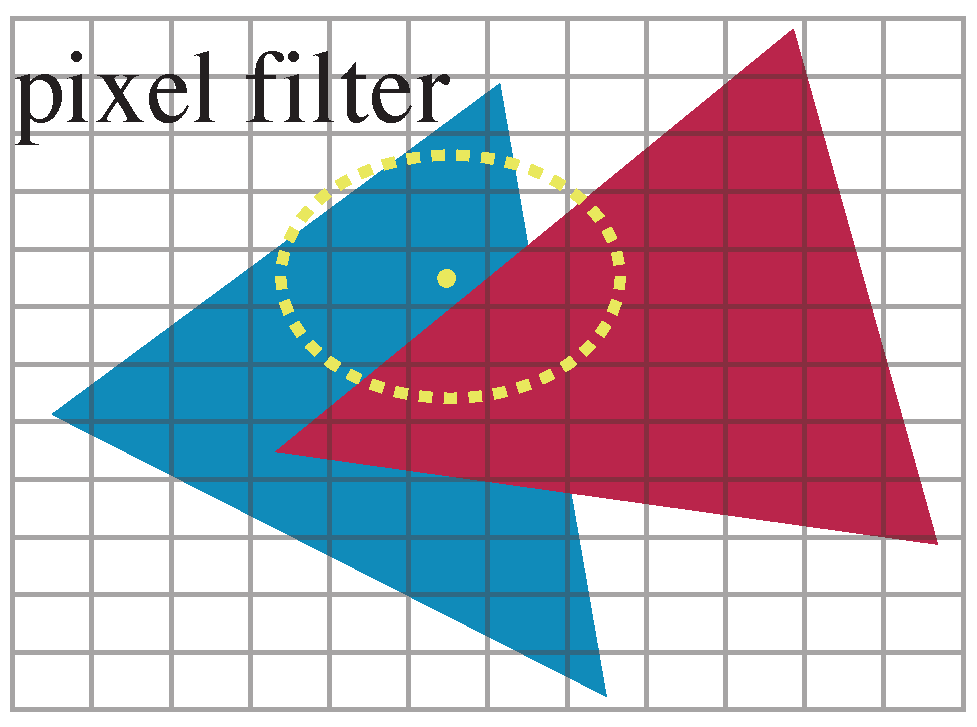
\includegraphics[width=0.4\linewidth]{imgs/pixel_filter.pdf}
    \includegraphics[width=0.4\linewidth]{imgs/antialiasing.pdf}
    \caption{To reconstruct the continuous scene from the discrete pixel samples, the color of a pixel is computed by integrating over a \emph{pixel filter}.}
    \label{fig:pixel_filter}
\end{figure}

\begin{figure}[h]
    \centering
    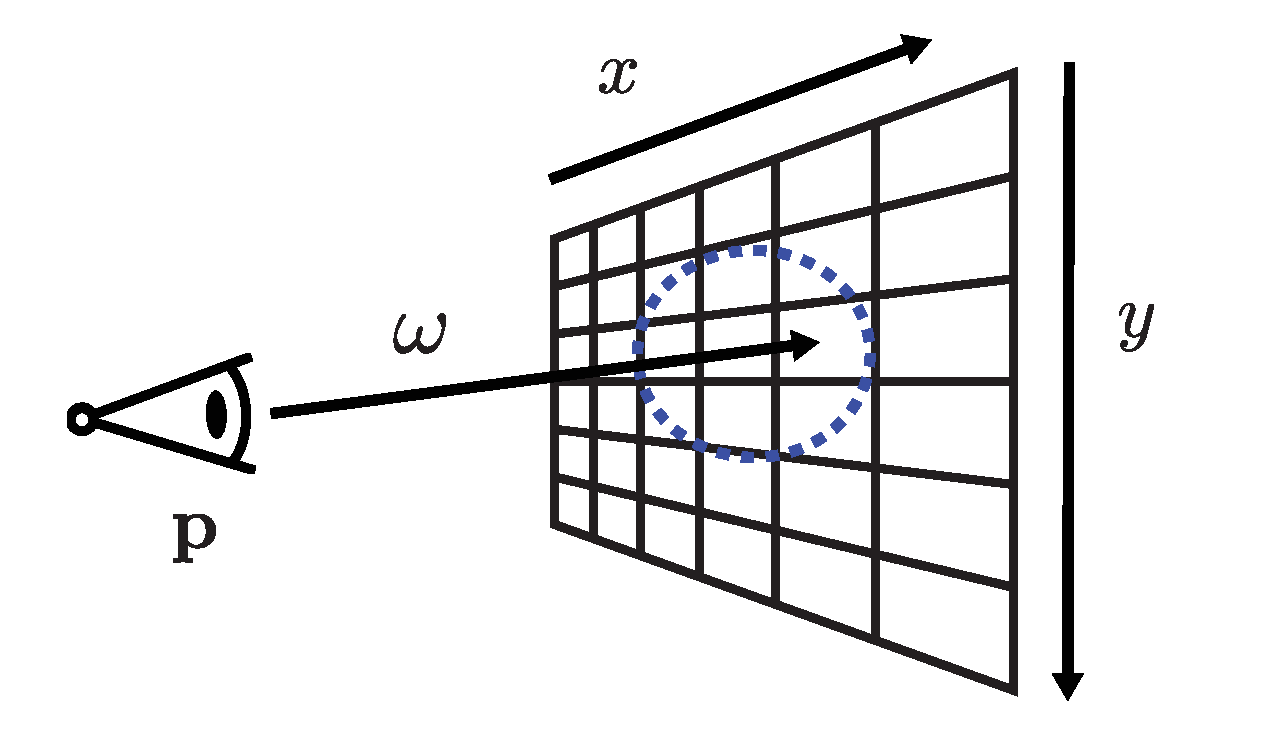
\includegraphics[width=0.4\linewidth]{imgs/camera.pdf}
    \caption{Camera configuration and pixel filtering.}
    \label{fig:camera}
\end{figure}

How does lajolla, or many other modern physically-based renderer compute the color for each pixel? They do this by \emph{integrating} all lights that go through a pixel. Note that a pixel is not an infinitesimal point, nor is it a little square~\cite{Smith:1995:PLS}. \textbf{A pixel is a reconstruction filter over an image function at a certain location} (Figure~\ref{fig:pixel_filter}). Mathematically, a pixel $I_{x, y}$'s color is written as a filtering integral:
\begin{equation}
    I_{x, y} = \iint_{D} k(x', y') L(\mathbf{p}, \mathbf{\omega}(x + x', y + y')) \mathrm{d}x\mathrm{d}y,
    \label{eq:pixel_filter}
\end{equation}
where $k$ is the \emph{filter kernel}, $D$ is the \emph{support} of the filter kernel (the pixel location where its value is non-zero), and $L(\mathbf{p}, \mathbf{\omega})$ is the radiance at point $\mathbf{p}$, received from direction $\mathbf{\omega}$ where the direction is pointing outwards from $\mathbf{p}$. In our case, $\mathbf{p}$ is the position of the camera, and $\mathbf{\omega}$ is the direction between the camera position and the points on the film (Figure~\ref{fig:camera}).

Now we have three questions: 1) what is the filter kernel $k$? 2) what is the radiance $L$?, and 3) how do we evaluate this integral on a computer? For 1), we will discuss a bit more in Section~\ref{sec:pixel_filter}, but for now you can think of it as something like a 2D Gaussian. For 3), these integrals typically do not have closed-form solutions,\footnote{There are rendering algorithms that are based on closed-form solutions of these integrals. Some radiosity algorithms~\cite{Schroder:1993:OFF} make use of closed-form solutions, for example. Also check out the excellent paper from Heitz et al.~\cite{Heitz:2016:RPS}} so we need to \emph{discretize} these integrals:
\begin{equation}
    \int_{D} F(x) dx \approx \frac{1}{N} \sum_{i=1}^{N} F(x_i),
    \label{eq:discretization}
\end{equation}
where $x_i$ are samples in uniform measures drawn from the domain $D$. When $x_i$ are random samples, this is called \emph{Monte Carlo} integration.\footnote{Monte Carlo integration was first invented for numerical simulation of nuclear weapons. Nicholas Metropolis, a member of the Manhattan Project, suggested the name to the simulation guy Stanislaw Ulam since Ulam's uncle likes to go to Monte Carlo for gambling.} However, $x_i$ does not need to be random. It can be deterministic samples that just somewhat uniformly cover the domain. When $x_i$ are deterministic, this approximation is often called \emph{quadrature} or \emph{cubature}. There is another class of deterministic integration methods called \emph{Quasi Monte Carlo} methods, which is based on the idea of carefully placing samples to make sure they are not far away from each other. We will cover these in the class if time permits.

\begin{figure}[h]
    \centering
    \includegraphics[width=0.4\linewidth]{imgs/pathtracing.pdf}
    \caption{The illustration of the rendering equation.}
    \label{fig:pathtracing}
\end{figure}

We are still left with Q2: what is the radiance $L$? In this class, we are mostly dealing with objects that are larger than the wavelength of lights. So under Newtonian optics, the radiance is simply the radiance $L_i$ at the object we see:
\begin{equation}
    L(\mathbf{p}, \mathbf{\omega}) = L_i(\mathbf{p}', -\mathbf{\omega}),
\end{equation}
where $\mathbf{p}'$ is the point the direction $\mathbf{\omega}$ intersect with the scene. Then -- what is $L_i$? An object is lit by a light source. However, as photons scatter between objects, a photon can first hit object A before it hits object B. Therefore, we need to recursively consider all objects in the scene (Figure~\ref{fig:pathtracing}):
\begin{equation}
    L_i(\mathbf{p}, \mathbf{\omega}) = L_e(\mathbf{p}, \mathbf{\omega}) + \int_{\Omega} f(\mathbf{p}, \mathbf{\omega}, \mathbf{\omega}') |\mathbf{n}_{\mathbf{p}} \cdot \mathbf{\omega}'| L_i(\mathbf{p}', -\mathbf{\omega}') \mathrm{d} \mathbf{\omega}',
    \label{eq:rendering_equation}
\end{equation}
where $L_e$ is the \emph{emission} at $\mathbf{p}$ towards direction $\mathbf{\omega}$, $\Omega$ is a spherical domain around point $\mathbf{p}$, $f$ is the reflectance of the object at point $p$ from direction $\mathbf{\omega}'$ to $\mathbf{\omega}$, $\mathbf{p}'$ is the point intersected by the ray $(\mathbf{p}, \mathbf{\omega}')$, and $n_{p}$. $f$ is often called the Bidirectional Scattering Distribution Function (BSDF) -- when the material is transmissive, it's called the Bidirectional Transmission Distribution Function (BTDF), and when it is reflective, it's called the Bidirectional Reflectance Distribution Function (BRDF) (I know, it's confusing). The measure $\mathrm{d} \mathbf{\omega}'$ is the \emph{solid angle}: the infinitesimal area on a unit sphere. Equation~\ref{eq:rendering_equation} is often called the \emph{rendering equation}~\cite{Kajiya:1986:RE}.

This recursive integral, combined with the integral discretization (Equation~\ref{eq:discretization}), gives us a rendering algorithm. We start from a pixel $(x, y)$, and sample a pixel offset $(x', y')$ to estimate the pixel filter integral (Equation~\ref{eq:pixel_filter}). Next, to estimate $L_i$, we sample a direction $\mathrm{d}'$, hit point $\mathbf{p}'$, multiply by $f$, and add $L_e$ whenever we hit a light source. In lajolla, the \lstinline{path_tracing} function in \lstinline{path_tracing.h} implements a slightly more sophisticated version of this. In below we describe those improvements.

\subsection{Importance sampling}
The naive algorithm above is correct, but can be inefficient. Consider a special case of the rendering equation, where we only recurse once:
\begin{equation}
    L_i(\mathbf{p}, \omega) = L_e(\mathbf{p}, \mathbf{\omega}) + \int_{\Omega} f(\mathbf{p}, \mathbf{\omega}, \mathbf{\omega}') |\mathbf{n}_{\mathbf{p}} \cdot \mathbf{\omega}'| L_e(\mathbf{p}', -\mathbf{\omega}') \mathrm{d} \mathbf{\omega}'.
\end{equation}
The only difference is that instead of $L_i$ in the integral that recursively integrates over all the other surfaces, we only consider the light source contribution $L_e$. Remember that we approximate the integral using a discrete sum. Suppose we randomly sample a direction on a sphere:
\begin{equation}
  \int_{\Omega} f(\mathbf{p}, \mathbf{\omega}, \mathbf{\omega}') |\mathbf{n}_{\mathbf{p}} \cdot \mathbf{\omega}'| L_e(\mathbf{p}', -\mathbf{\omega}') \mathrm{d} \mathbf{\omega} \approx \frac{1}{N} \frac{1}{\frac{1}{4 \pi}} \sum_{i}^{N} f(\mathbf{p}, \mathbf{\omega}, \mathbf{\omega}_i') |\mathbf{n}_{\mathbf{p}} \cdot \mathbf{\omega}_i'| L_e(\mathbf{p}', -\mathbf{\omega}_i').
\end{equation}
The $\frac{1}{\frac{1}{4\pi}}$ factor accounts for the uniform measure on a unit sphere. The variance of this sum can be really high if $N$ is not large enough: firstly, not every surface in the scene emits light, so only a small fraction of samples would have non-zero $L_e$. Secondly, our sampling does not take the BSDF $f$ into consideration: $f$ can have high variation between different samples.

Fortunately, there is a way to make this sampling more efficient. The key is to apply a change of variable to our integral. Let's focus on the emission $L_e$ first. Instead of blindly sampling a direction on the sphere, we can directly pick a point on the light source, then choose a direction towards that point. So instead of integrating over the direction $\mathbf{\omega}$, we apply a change of variable to instead integrate over the points $\mathbf{p}'$ that emit lights:
\begin{equation}
    \int_{\Omega} f(\mathbf{p}, \mathbf{\omega}, \mathbf{\omega}') |\mathbf{n}_{\mathbf{p}} \cdot \mathbf{\omega}'| L_e(\mathbf{p}', -\mathbf{\omega}') \mathrm{d} \mathbf{\omega} =
    \int_{E} f(\mathbf{p}, \mathbf{\omega}, \mathbf{\omega}'(\mathbf{p}')) |\mathbf{n}_{\mathbf{p}} \cdot \mathbf{\omega}'| L_e(\mathbf{p}', -\mathbf{\omega}') G(\mathbf{p}, \mathbf{p}') \mathrm{d} \mathbf{p}',
    \label{eq:next_event_estimation}
\end{equation}
where $E$ is the area of all light sources, and $G$ is the Jacobian of the variable reparametrization (often called the \emph{geometry term}). Using some geometry insights, we can derive that $G(\mathbf{p}, \mathbf{p}') = \frac{|\mathbf{n}_{\mathbf{p}'} \cdot \mathbf{\omega}'|}{\|\mathbf{p} - \mathbf{p}'\|^2} V(\mathbf{p}, \mathbf{p}')$, where $V(\mathbf{p}, \mathbf{p}')$ is the \emph{visibility function} where $V=1$ if $\mathbf{p}$ can see $\mathbf{p}'$ and $V=0$ if they are occluded. Intuitively, $G$ is the area ratio of an infinitesimal area projected onto an unit sphere.

When the light source is visible for most of the time, the discretization of the second integral is much more efficient at locating lights since we focus on the domain $E$ instead of the whole spherical domain.

We can similarly account for the BSDF $f$ and the cosine $|\mathbf{n}_{\mathbf{p}} \cdot \mathbf{\omega}'|$ using a similar change of variable trick. This change of variable is often called \emph{importance sampling}. The particular change of variable trick above (Equation~\ref{eq:next_event_estimation}) is called the \emph{next event estimation}.

In general, for a (potentially multi-dimensional) integral $\int g(x) \mathrm{d}x$, we can rewrite it using a change of variable $y = T(x)$, where $T$ is an invertible function. This gives us $\int g(T^{-1}(y)) \frac{1}{|\frac{\mathrm{d}y}{\mathrm{d}x}|} \mathrm{d}y$, where $|\frac{\mathrm{d}y}{\mathrm{d}x}|$ is the Jacobian of the mapping $T$. If we discretize the new integral using uniform samples $y_i$, then we can see the new discretization as drawing samples $x_i = T^{-1}(y_i)$, evaluate $g(x_i)$, then weight them with the inverse of the Jacobian $|\frac{\mathrm{d}y}{\mathrm{d}x}|$ (as opposed to drawing $x_i$ as uniform samples and weight them with $1$). The Jacobian can be seen as the \emph{probability density function} of the samples $x_i = T^{-1}(y_i)$ (since the probability density function needs to integrate to $1$, we are essentially applying a change of variable for that integral too). 

In lajolla, the \lstinline{sample_light} and \lstinline{sample_point_on_light} functions implement the light source sampling strategy above. \lstinline{sample_light} pick a light source (from many) proportional to their relative powers, and \lstinline{sample_point_on_light} pick a point on the selected light source. \lstinline{light_pmf} and \lstinline{pdf_point_on_light} are the probability density (or probability mass function in the case of discrete distributions) of the corresponding sampling operations. Similarly, \lstinline{sample_bsdf} samples a direction that is proportional to $f$, and \lstinline{pdf_sample_bsdf} is the corresponding probability density.

\subsection{Multiple importance sampling}

If we have multiple change of variables we want to apply (e.g., sampling from lights and sampling from BSDFs), how do we combine them? One (inefficient) way to do this is to combine them by averaging the results. For example, for an integral $\int g(x) \mathrm{d}x$, we can apply $y = T_1(x)$ and $z = T_2(x)$, and evaluate $\frac{g(x(y_i))}{\left|
\frac{\mathrm{d}T_1}{\mathrm{d}x}\right|}$ and $\frac{g(x(z_i))}{\left|\frac{\mathrm{d}T_2}{\mathrm{d}x}\right|}$. We can approximate the integral as
\begin{equation}
\frac{1}{N} \sum
\frac{1}{2} \frac{g(x(y_i))}{\left|\frac{\mathrm{d}T_1}{\mathrm{d}x}(x(y_i))\right|} + 
\frac{1}{2} \frac{g(x(z_i))}{\left|\frac{\mathrm{d}T_2}{\mathrm{d}x}(x(z_i))\right|}.
\end{equation}

This is, however, not a great idea. If one of our sampling transformations has high variance, even if the other one achieves zero variance, this resulting estimator would still have a very high variance.

Eric Veach made a breakthrough in physically-based rendering by figuring out how we combine different estimators~\cite{Veach:1995:OCS}. The idea is to apply higher weight for the \emph{better} estimator. How do we know which estimator is better? We look at the Jacobian $|\frac{\mathrm{d}T}{\mathrm{d}x}(x)|$, or equivalently the probability density: if the Jacobian is high, that means that our sampling strategy has high sampling density around $x_i$ -- which means it's more efficient around that area. We can weigh the samples using the corresponding Jacobian:
\begin{equation}
\frac{1}{N} \sum
\frac{\left|\frac{\mathrm{d}T_1}{\mathrm{d}x}(x(y_i))\right|}{\left|\frac{\mathrm{d}T_1}{\mathrm{d}x}(x(y_i))\right| + \left|\frac{\mathrm{d}T_2}{\mathrm{d}x}(x(y_i))\right|}
\frac{g(x(y_i))}{\left|\frac{\mathrm{d}T_1}{\mathrm{d}x}(x(y_i))\right|} + 
\frac{\left|\frac{\mathrm{d}T_2}{\mathrm{d}x}(x(z_i))\right|}{\left|\frac{\mathrm{d}T_1}{\mathrm{d}x}(x(z_i))\right| + \left|\frac{\mathrm{d}T_2}{\mathrm{d}x}(x(z_i))\right|}
\frac{g(x(z_i))}{\left|\frac{\mathrm{d}T_2}{\mathrm{d}x}(x(z_i))\right|}.
\end{equation}
Note that there are four different Jacobians here: $\left|\frac{\mathrm{d}T_1}{\mathrm{d}x}(x(y_i))\right|$, $\left|\frac{\mathrm{d}T_2}{\mathrm{d}x}(x(y_i))\right|$, $\left|\frac{\mathrm{d}T_1}{\mathrm{d}x}(x(z_i))\right|$, and $\left|\frac{\mathrm{d}T_2}{\mathrm{d}x}(x(z_i))\right|$.

Alternatively, Veach also proposed another weight called the \emph{power heuristics} that put even more emphasis on strategies with high Jacobian values:
\begin{equation}
\frac{1}{N} \sum
\frac{\left|\frac{\mathrm{d}T_1}{\mathrm{d}x}(x(y_i))\right|^2}{\left|\frac{\mathrm{d}T_1}{\mathrm{d}x}(x(y_i))\right|^2 + \left|\frac{\mathrm{d}T_2}{\mathrm{d}x}(x(y_i))\right|^2}
\frac{g(x(y_i))}{|\frac{\mathrm{d}T_1}{\mathrm{d}x}(x(y_i))|} + 
\frac{\left|\frac{\mathrm{d}T_2}{\mathrm{d}x}(x(z_i))\right|^2}{\left|\frac{\mathrm{d}T_1}{\mathrm{d}x}(x(z_i))\right|^2 + \left|\frac{\mathrm{d}T_2}{\mathrm{d}x}(x(z_i))\right|^2}
\frac{g(x(z_i))}{\left|\frac{\mathrm{d}T_2}{\mathrm{d}x}(x(z_i))\right|}.
\end{equation}

Veach made more justification of the method in his paper (which I highly recommend you to read!). However, note that these are ultimately ``heuristics'', and they can be suboptimal in certain cases. Finding better multiple importance sampling weights is an active research area.

lajolla uses the power heuristics for combining different strategies.

\paragraph{The path-space integral.} The rendering equation above is a recursive equation, and while recursion is cool, it's often easier to analyze and understand its structure if we can flatten it to a more iterative form. By expanding the recursion, we see the following pattern
\begin{equation}
    L_i = L_e + f * L_e + f * f * L_e + \dots.
\end{equation}
We notice that we are essentially tracing \emph{light paths} with a different number of vertices. For light paths with two vertices: one at the camera position and one at a light source, we only need to compute $L_e$. For light paths with three vertices, we need to account for one scattering event and multiply $f$. If we define a light path with a sequence of directions: $\mathbf{D} = ((x', y'), \mathbf{\omega}_1, \mathbf{\omega}_2, \dots)$, then we can define a \emph{path contribution function} $f_d$ to compute the contribution of that single light path. From above, we can see that
\begin{equation}
    f_d(\mathbf{D}) = k(x', y') f(\mathbf{p}_1, \mathbf{\omega}_0(x', y'), \mathbf{\omega}_1) f(\mathbf{p}_2, \mathbf{\omega}_1, \mathbf{\omega}_2) \dots L_e(\mathbf{p}_N, \mathbf{\omega}_N).
\end{equation}
(I might have got some signs wrong but don't worry about it.)

We can then rewrite the rendering integral as
\begin{equation}
    I_{x, y} = \int f_d(\mathbf{D}) \mathrm{d} D(\mathbf{\omega}),
\end{equation}
where the measure $D(\mathbf{\omega})$ is the product of solid angle of the path directions $\mathbf{\omega}_i$.

A path can also be written in many different forms. A very convenient form is to define the path as a sequence of positions, as opposed of directions: $\mathbf{P} = (\mathbf{p}_0, \mathbf{p}_1, \mathbf{p}_2, \dots)$. While these two forms are equivalent, this again is a change of variable. The new path contribution function $f_p(\mathbf{P})$ is:
\begin{equation}
    f_p(\mathbf{P}) = k((x', y')(\mathbf{p}_0, \mathbf{p_1})) G_0(\mathbf{p}_0, \mathbf{p}_1) f(\mathbf{p}_1, \mathbf{\omega}_0, \mathbf{\omega}_1)G(\mathbf{p}_1, \mathbf{p}_2) f(\mathbf{p}_2, \mathbf{\omega}_1, \mathbf{\omega}_2) \dots G(\mathbf{p}_{N-1}, \mathbf{p}_{N}) L_e(\mathbf{p}_N, \mathbf{\omega}_N),
\end{equation}
where $G$ is again the geometry term that accounts for the Jacobian. The first geometry term $G_0$ is slightly more complicated as it is the Jacobian between $\mathbf{p}_1$ and pixel integral variables $x', y'$. We don't need it here yet, so don't worry about it.

This path integral enables a more principled way to think about rendering algorithms. For example, we do not need to always trace paths from the cameras. We can trace paths from lights and it still gives us a valid light path. We can even just randomly sample spatial location to construct a sequence of positions $\mathbf{p}$.

\section{Camera}

Lajolla implements a fairly standard pinhole perspective camera:
\begin{lstlisting}[language=c++]
struct Camera {
    Camera() {}
    Camera(const Matrix4x4 &cam_to_world,
           Real fov, // in degree
           int width, int height,
           const Filter &filter,
           int medium_id);

    Matrix4x4 sample_to_cam, cam_to_sample;
    Matrix4x4 cam_to_world, world_to_cam;
    int width, height;
    Filter filter;

    int medium_id; // for participating media rendering in homework 2
};
\end{lstlisting}
The matrices transform a 2D pixel location $(x, y)$ to a ray direction $\omega$. The \lstinline{sample_primary} function implements the functionality for sampling a ray given a screen position.
\begin{lstlisting}[language=c++]
/// Given screen position in [0, 1] x [0, 1], generate a camera ray.
Ray sample_primary(const Camera &camera,
                   const Vector2 &screen_pos);
\end{lstlisting}

\subsection{Pixel filter}
\label{sec:pixel_filter}

\begin{figure}
    \centering
    \begin{subfigure}[t]{0.32\linewidth}
        \centering
        \includegraphics[width=\textwidth]{imgs/box.png}
        \caption{box}
        \label{fig:box_filter}
    \end{subfigure}
    \begin{subfigure}[t]{0.32\linewidth}
        \centering
        \includegraphics[width=\textwidth]{imgs/tent.png}
        \caption{tent}
        \label{fig:tent_filter}
    \end{subfigure}
    \begin{subfigure}[t]{0.32\linewidth}
        \centering
        \includegraphics[width=\textwidth]{imgs/gaussian.png}
        \caption{Gaussian ($\sigma = 0.75$)}
        \label{fig:gaussian_filter}
    \end{subfigure}
    \caption{A poor pixel filter can lead to the \emph{aliasing} artifact: high-frequency signals ``leak'' into the reconstruction and we see patterns that should not exist (zoom in and observe the top part of the images). Blurring the signal resolves this issue: the design of a good pixel filter trades between aliasing, blurriness, and ringing (oversharpening).\protect\footnotemark}
    \label{fig:pixel_filter_comp}
\end{figure}

A crucial component of the camera is the \emph{pixel filter}, which corresponds to the $k$ kernel above. As we have emphasized: \textbf{a pixel is not a little square}. It is a reconstruction from a discrete sampling of a continuous underlying signal. The choice of the reconstruction filter/kernel can have a significant impact on the quality of the reconstruction. A naive box filter can suffer from severe \emph{aliasing} effects, since its Fourier transform is a sinc function that can have negative weights in the frequency domain and high-frequency energy. Lajolla currently supports three different filters (Figure~\ref{fig:pixel_filter_comp}):\footnotetext{In this particular case, a proper texture prefiltering should give a better result, but checkerboard texture filtering has not been implemented in lajolla.}

\begin{lstlisting}[language=c++]
struct Box {
    Real width;
};
struct Tent {
    Real width;
};
struct Gaussian {
    Real stddev;
};
using Filter = std::variant<Box, Tent, Gaussian>;
\end{lstlisting}

Lajolla implements pixel filtering in a slightly different way compared to other open-source renderes such as Mitsuba or pbrt. Many common open-source renderers implement pixel filtering using a "splatting" approach: they sample a point from a pixel, and then splat the contribution to all nearby pixels overlapped with the filter support. This approach works fine, but has a few disadvantages:
\begin{itemize}
    \item This introduces race conditions between different pixels, and requires atomic operations.
    \item This introduces correlation between pixels and hurts denoising.
    \item The splatting approach is biased and creates artifacts at low sampling rates.
    \item For filters with infinite supports (e.g., Gaussian), this requires a discontinuous cutoff radius (otherwise it would be too slow).
\end{itemize}
For these reasons, many modern production renderers have started to employ a different and simpler strategy. For each pixel, we solve for the pixel filter integral by directly importance sample that filter, and we *do not* share samples among pixels. This allows us to avoid all three problems above. This approach was described by Shirley et al. in 1991~\cite{Shirley:1991:RTF} and was discussed more recently by Ernst et al.~\cite{Ernst:2006:FIS}.

\begin{lstlisting}[language=c++]
Vector2 sample(const Filter &filter, const Vector2 &rnd_param);

Vector2 sample_op::operator()(const Box &filter) const {
    // Warp [0, 1]^2 to [-width/2, width/2]^2
    return (Real(2) * rnd_param - Real(1)) * (filter.width / 2);
}

Vector2 sample_op::operator()(const Tent &filter) const {
    // See comments in code for more explanation.
    Real h = filter.width / 2;
    Real x = rnd_param[0] < 0.5 ? 
        h * (sqrt(2 * rnd_param[0]) - 1) :
        h * (1 - sqrt(1 - 2 * (rnd_param[0] - Real(0.5))));
    Real y = rnd_param[1] < 0.5 ? 
        h * (sqrt(2 * rnd_param[1]) - 1) :
        h * (1 - sqrt(1 - 2 * (rnd_param[1] - Real(0.5))));
    return Vector2{x, y};
}

Vector2 sample_op::operator()(const Gaussian &filter) const {
    // Box Muller transform
    // https://en.wikipedia.org/wiki/Box%E2%80%93Muller_transform
    Real r = filter.stddev * sqrt(-2 * log(max(rnd_param[0], 1e-8)));
    return Vector2{r * cos(2 * c_PI * rnd_param[1]),
                   r * sin(2 * c_PI * rnd_param[1])};
}

Ray sample_primary(const Camera &camera,
                   const Vector2 &screen_pos) {
    // screen_pos' domain is [0, 1]^2
    Vector2 pixel_pos{screen_pos.x * camera.width, screen_pos.y * camera.height};

    // Importance sample from the pixel filter (see filter.h for more explanation).
    // We first extract the subpixel offset.
    Real dx = pixel_pos.x - floor(pixel_pos.x);
    Real dy = pixel_pos.y - floor(pixel_pos.y);
    // dx/dy are uniform variables in [0, 1],
    // so let's remap them using importance sampling.
    Vector2 offset = sample(camera.filter, Vector2{dx, dy});
    // Filters are placed at pixel centers.
    Vector2 remapped_pos{
      (floor(pixel_pos.x) + Real(0.5) + offset.x) / camera.width,
      (floor(pixel_pos.y) + Real(0.5) + offset.y) / camera.height};

    Vector3 pt = xform_point(camera.sample_to_cam,
        Vector3(remapped_pos[0], remapped_pos[1], Real(0)));
    Vector3 dir = normalize(pt);
    return Ray{xform_point(camera.cam_to_world, Vector3{0, 0, 0}),
               // the last normalize might not be necessary
               normalize(xform_vector(camera.cam_to_world, dir)),
               Real(0), infinity<Real>()};
}
\end{lstlisting}

\section{Materials}
\begin{figure}
    \centering
    \begin{subfigure}[t]{0.32\linewidth}
        \centering
        \begin{minipage}[t]{\linewidth}
            \includegraphics[width=\linewidth]{imgs/lambertian_render.png}
            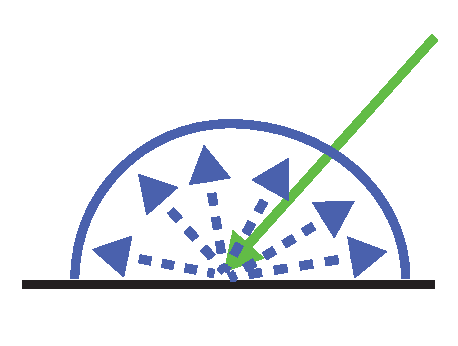
\includegraphics[width=\linewidth]{imgs/lambertian.pdf}
        \end{minipage}
        \caption{Lambertian}
        \label{fig:lambertian}
    \end{subfigure}
    \begin{subfigure}[t]{0.32\linewidth}
        \centering
        \begin{minipage}[t]{\linewidth}
            \includegraphics[width=\linewidth]{imgs/roughplastic_render.png}
            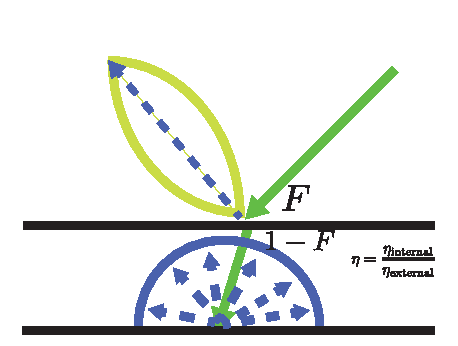
\includegraphics[width=\linewidth]{imgs/roughplastic.pdf}
        \end{minipage}
        \caption{rough plastic}
        \label{fig:rough_plastic}
    \end{subfigure}
    \begin{subfigure}[t]{0.32\linewidth}
        \centering
        \begin{minipage}[t]{\linewidth}
            \includegraphics[width=\linewidth]{imgs/roughdielectric_render.png}
            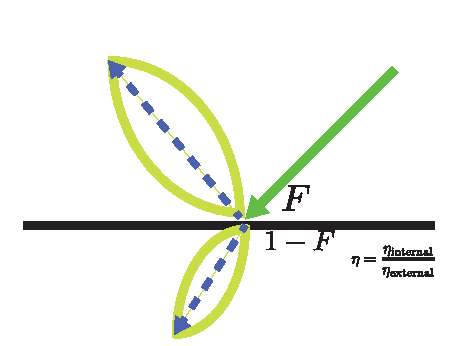
\includegraphics[width=\linewidth]{imgs/roughdielectric.pdf}
        \end{minipage}
        \caption{rough dielectric}
        \label{fig:rough_dielectric}
    \end{subfigure}
    \caption{Three materials lajolla supports currently. Lambertian is a diffusive material that reflects light uniformly. Rough plastic is a two-layer material with a dielectric coating at the top, and a diffusive material at the bottom. The Fresnel equation $F$ determines how much lights are reflected, and how much are refracted into the diffusive material. If the light is reflected at the dielectric layer, a distribution centered at the mirror reflection angle determined by the microfacet theory~\cite{Cook:1982:RMC} is used. If the light is reflected through the dielectric layer, a Lambertian response is used, attenuated by the Fresnel reflection. Finally, the rough dielectric material is similar to the dielectric layer of rough plastic, but it refracts light by an amount predicted by the Fresnel equation.}
    \label{fig:materials}
\end{figure}

Recall that in the rendering equation, we need the BSDF $f$ for describing how objects reflect or refract lights. Designing and capturing BSDFs is a large field of study, and we will cover some of them in this course. Lajolla currently supports three different materials/BSDFs (and you will implement a few more in the next homework!):
\begin{lstlisting}[language=c++]
struct Lambertian {
    Texture<Spectrum> reflectance;
};

struct RoughPlastic {
    Texture<Spectrum> diffuse_reflectance;
    Texture<Spectrum> specular_reflectance;
    Texture<Real> roughness;

    // Note that the material is not transmissive.
    // This is for the IOR between the dielectric layer and the diffuse layer.
    Real eta; // internal IOR / externalIOR
};

struct RoughDielectric {
    Texture<Spectrum> specular_reflectance;
    Texture<Spectrum> specular_transmittance;
    Texture<Real> roughness;

    Real eta; // internal IOR / externalIOR
};
\end{lstlisting}

See Figure~\ref{fig:materials} for an explanation of the three materials. While we will cover them in the course, I highly recommend Cook and Torrance's seminal paper~\cite{Cook:1982:RMC} for a primer of the microfacet-based BSDFs. You should also read Walter's paper on extending Cook and Torrance's model to handle refraction~\cite{Walter:2007:MMR}.

\paragraph{Material interfaces.} Every material in lajolla needs to implement the following functions:
\begin{lstlisting}[language=c++]
/// Given incoming direction and outgoing direction of lights,
/// both pointing outwards of the surface point,
/// outputs the BSDF times the cosine between outgoing direction
/// and the shading normal, evaluated at a point.
/// When the transport direction is towards the lights,
/// dir_in is the view direction, and dir_out is the light direction.
/// Vice versa.
Spectrum eval(const Material &material,
              const Vector3 &dir_in,
              const Vector3 &dir_out,
              const PathVertex &vertex,
              const TexturePool &texture_pool,
              TransportDirection dir = TransportDirection::TO_LIGHT);

struct BSDFSampleRecord {
    Vector3 dir_out;
    // The index of refraction ratio. Set to 0 if it's not a transmission event.
    Real eta;
    Real roughness; // Roughness of the selected BRDF layer ([0, 1]).
};

/// Given incoming direction pointing outwards of the surface point,
/// samples an outgoing direction. Also returns the index of refraction
/// and the roughness of the selected BSDF layer for path tracer's use.
/// failed (e.g., if the incoming direction is invalid).
/// If dir == TO_LIGHT, incoming direction is the view direction and 
/// we're sampling for the light direction. Vice versa.
std::optional<BSDFSampleRecord> sample_bsdf(
    const Material &material,
    const Vector3 &dir_in,
    const PathVertex &vertex,
    const TexturePool &texture_pool,
    const Vector2 &rnd_param_uv,
    const Real &rnd_param_w,
    TransportDirection dir = TransportDirection::TO_LIGHT);

/// Given incoming direction and outgoing direction of lights,
/// both pointing outwards of the surface point,
/// outputs the probability density of sampling.
/// If dir == TO_LIGHT, incoming direction is dir_view and 
/// we're sampling for dir_light. Vice versa.
Real pdf_sample_bsdf(const Material &material,
                     const Vector3 &dir_in,
                     const Vector3 &dir_out,
                     const PathVertex &vertex,
                     const TexturePool &texture_pool,
                     TransportDirection dir = TransportDirection::TO_LIGHT);

/// Return a texture from the material for debugging.
/// If the material contains multiple textures, return an arbitrary one.
TextureSpectrum get_texture(const Material &material);
\end{lstlisting}

The comments should be self-explanatory. If they are not, let us know. Note that in lajolla, the BSDF functions also contain the cosine term $|\mathbf{n}_{\mathbf{p}} \cdot \omega'|$: this makes the overall code simpler. \textbf{For the homework, you do not need to worry about \lstinline{TransportDirection}: you can assume they are always pointing towards the lights.} This is for convenience for implementing a bidirectional path tracer.

\subsection{Textures and filtering}
Almost all values of material should be spatially varying. Textures are a way to describe these spatially varying materials using a 2D function: given a 2D coordinates $(u, v)$, a texture maps it to a value $T$ (can be a color or just a real number). There are three kinds of textures in lajolla currently:

\begin{lstlisting}[language=c++]
template <typename T>
struct ConstantTexture {
    T value;
};

template <typename T>
struct ImageTexture {
    int texture_id;
    Real uscale, vscale;
    Real uoffset, voffset;
};

template <typename T>
struct CheckerboardTexture {
    T color0, color1;
    Real uscale, vscale;
    Real uoffset, voffset;
};

template <typename T>
using Texture = std::variant<ConstantTexture<T>, ImageTexture<T>, CheckerboardTexture<T>>;
using Texture1 = Texture<Real>;
using TextureSpectrum = Texture<Spectrum>;

/// Evaluate the texture at location uv.
/// Footprint should be approximatedly min(du/dx, du/dy, dv/dx, dv/dy) for texture filtering.
template <typename T>
T eval(const Texture<T> &texture, const Vector2 &uv, Real footprint, const TexturePool &pool);
\end{lstlisting}

In lajolla, all surfaces must come with a 2D $(u, v)$ parametrization. We use this 2D $uv$ vector $(\in [0, 1]^2)$ for accessing the textures. A constant texture uses a constant value for all $uv$. An image texture loads an image from a file and uses it to represent the texture. A checkerboard texture is a procedural texture that outputs a checkerboard pattern (see Figure~\ref{fig:pixel_filter_comp} for example).

\begin{figure}
    \centering
    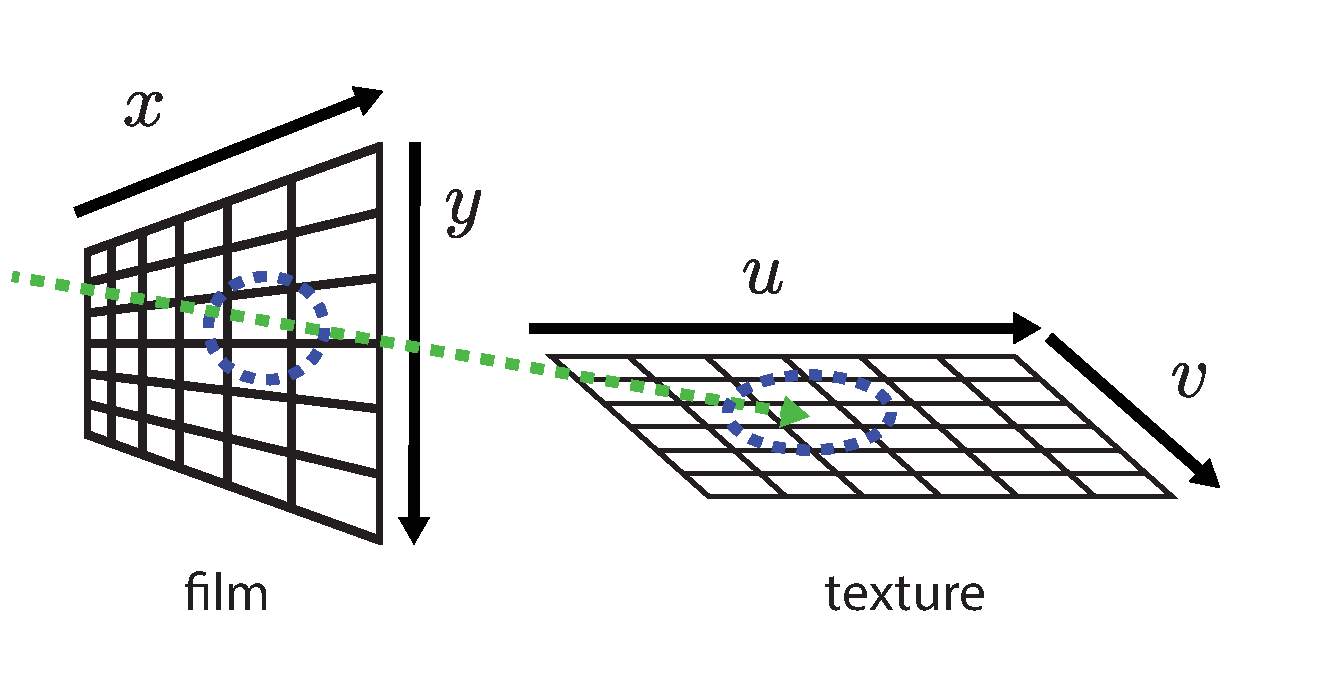
\includegraphics[width=0.4\linewidth]{imgs/texture_filtering.pdf}
    \caption{The pixel footprint will propagate to texture access, requiring us to access a large region of the texture. The size of the ellipse on the texture is determined by the derivative $\frac{\mathrm{d}u}{\mathrm{d}x}, \frac{\mathrm{d}u}{\mathrm{d}y}, \frac{\mathrm{d}v}{\mathrm{d}x},$ and $\frac{\mathrm{d}v}{\mathrm{d}y}$.}
    \label{fig:texture_filtering}
\end{figure}

\begin{figure}
    \centering
    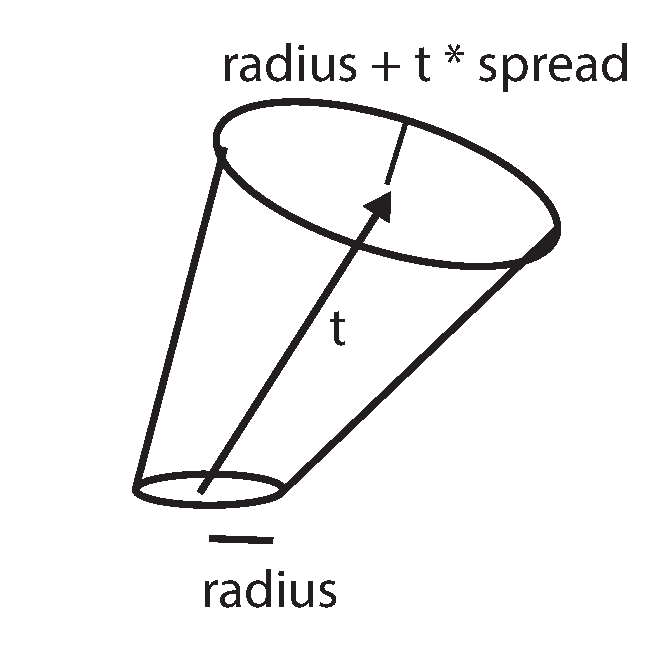
\includegraphics[width=0.3\linewidth]{imgs/ray_differential.pdf}
    \caption{We use a simplified and conservative ray differential adopted by RenderMan: a radius and a spread is maintained for each ray for determining the texture footprint.}
    \label{fig:ray_differential}
\end{figure}

\paragraph{Filtering and ray differentials.} Similar to the pixel filter, it is crucial that we filter the texture as well to avoid aliasing. When accessing a texture, we want to know the relative size between the filter on uv and the pixel filter (Figure~\ref{fig:texture_filtering}). This relative size is determined by the derivatives between $uv$ and $xy$. Note that we need to access textures for many bounces of lights, and it is difficult to estimate the texture footprint over many bounces. A commonly used method for determining texture footprint is the \emph{ray differentials}~\cite{Igehy:1999:TRD}, however it only works for purely specular materials. \emph{Path differentials}~\cite{Suykens:2001:PDA} is an extension of ray differential for glossy materials, but it is extremely expensive to compute. A slightly more principled way based on local Fourier analysis called covariance tracing~\cite{Belcour:2017:ACG} can propagate the Fourier spectrum of the pixel filter using a Gaussian approximation, but 1) it requires us to have knowledge of the Fourier spectrum of the BSDF, and 2) it is still an approximation because it ignores visibility. In general, if we ignore visibility, all existing methods would predict an infinite filter size if a light path goes through a diffuse bounce. However this is clearly incorrect, since object boundaries and visibility would limit the texture filter size. The existing approaches have to place a manually determined maximum filter size to prevent infinite filter size.

Since all existing methods are heuristics and there is really no satisfactory solution for multiple bounces (which means there is research to be done here!), we will use a very simple and conservative heuristic, inspired by the implementation in modern RenderMan~\cite{Christensen:2018:RAP} and an experimental branch of pbrt.\footnote{See \href{https://www.pbrt.org/texcache.pdf}{THE IMPLEMENTATION OF A SCALABLE TEXTURE CACHE} from Matt Pharr} We maintain two numbers for a ray differential: the \emph{radius} of a ray and a \emph{spread} of a ray (Figure~\ref{fig:ray_differential}) -- now that the ray becomes a \emph{ray cone} and the size of the cone can be used for determining the texture footprint. These values are approximately the derivative of the ray origin and ray direction with respect to the pixel coordinates.
\begin{lstlisting}[language=c++]
struct RayDifferential {
    // Radius is approximately (length(dp/dx) + length(dp/dy)) / 2
    // Spread is approximately (length(dd/dx) + length(dd/dy)) / 2
    // p is ray position, d is ray direction.
    Real radius = 0, spread = 0; // The units are pixels.
};
\end{lstlisting}

To initiailize a ray differential, we set it to $1/4$ the size of a pixel:
\begin{lstlisting}[language=c++]
inline RayDifferential init_ray_differential(int w, int h) {
    return RayDifferential{Real(0), Real(0.25) / max(w, h)};
}
\end{lstlisting}

To propagate a ray differential over a distance, we update the radius of the ray using its spread
\begin{lstlisting}[language=c++]
/// Update the radius (dp/dx) of a ray differential by propagating it over a distance.
inline Real transfer(const RayDifferential &r, Real dist) {
    return r.radius + r.spread * dist;
}
r.radius = transfer(r, dist);
\end{lstlisting}

To model a scattering event, we blend between the spread of a pure specular event and a spread of a diffuse event using the roughness of the material: roughness 0 corresponds to a pure specular event.
For a pure specular event, the amount of spread is determined by the curvature of a surface.
For the diffuse event, we manually set a cone size.
\begin{lstlisting}[language=c++]
/// Update the spread (dd/dx) of a ray differential by scattering over a reflective surface.
inline Real reflect(const RayDifferential &r,
                    Real mean_curvature,
                    Real roughness) {
    Real spec_spread = r.spread + 2 * mean_curvature * r.radius;
    Real diff_spread = Real(0.2);
    return fmax(spec_spread * (1 - roughness) + diff_spread * roughness, Real(0));
}
\end{lstlisting}

For refraction, we need to additionally take the index of refraction into account. According to Snell-Descartes law, the ray spread would change by the ratio of the index of refraction. If the ratio is large, rays will be more concentrated, and vice versa. So we just divide the spread with that ratio.
\begin{lstlisting}[language=c++]
/// Update the spread (dd/dx) of a ray differential by scattering over a reflective surface.
inline Real refract(const RayDifferential &r,
                    Real mean_curvature,
                    Real roughness) {
    Real spec_spread = (r.spread + 2 * mean_curvature * r.radius) / eta;
    Real diff_spread = Real(0.2);
    return fmax(spec_spread * (1 - roughness) + diff_spread * roughness, Real(0));
}
\end{lstlisting}
Note that these are all approximation and heuristics. Read the references above to see other alternatives as well.

Once we have the footprint of a ray radius (approximately $\frac{dp}{dx}$), we can convert it to the UV space using the derivative $\frac{du}{dp}$, which we can compute from the geometry quantities. This uv space footprint is then passed to the texture as the \lstinline{footprint} argument. We then want to filter the texture using a filter with support of \lstinline{footprint}. Looping over all texels inside the footprint is too slow. Therefore we precompute an \emph{image pyramid} of the texture for representing signals at different frequencies. This image pyramid is called the Mipmap. We can then reconstruct a value of a texture with a certain footprint, by linearly interpolating levels between a mipmap.

\begin{lstlisting}[language=c++]
template <typename T>
struct Mipmap {
    std::vector<Image<T>> images;
};

/// Bilinear lookup of a mipmap at location (uv) with an integer level
template <typename T>
inline T lookup(const Mipmap<T> &mipmap, Real x, Real y, int level);

/// Trilinear look of of a mipmap at (u, v, level)
template <typename T>
inline T lookup(const Mipmap<T> &mipmap, Real u, Real v, Real level) {
    if (level <= 0) {
        return lookup(mipmap, u, v, 0);
    } else if (level < Real(mipmap.images.size() - 1)) {
        int flevel = std::clamp((int)floor(level), 0, (int)mipmap.images.size() - 1);
        int clevel = std::clamp(flevel + 1, 0, (int)mipmap.images.size() - 1);
        Real level_off = level - flevel;
        return lookup(mipmap, u, v, flevel) * (1 - level_off) +
               lookup(mipmap, u, v, clevel) *      level_off;
    } else {
        return lookup(mipmap, u, v, int(mipmap.images.size() - 1));
    }
}
\end{lstlisting}

To determine the mipmap level, we just take a base 2 log of the footprint.
\begin{lstlisting}[language=c++]
template <typename T>
T eval_texture_op<T>::operator()(const ImageTexture<T> &t) const {
    const Mipmap<T> &img = get_img(t, pool);
    Vector2 local_uv{modulo(uv[0] * t.uscale + t.uoffset, Real(1)),
                     modulo(uv[1] * t.vscale + t.voffset, Real(1))};
    Real scaled_footprint = max(get_width(img), get_height(img)) * max(t.uscale, t.vscale) * footprint;
    Real level = log2(max(scaled_footprint, Real(1e-8f)));
    return lookup(img, local_uv[0], local_uv[1], level);
}
\end{lstlisting}

\paragraph{Texture Pool.} Modern production renderers do not actually load all textures to the memory when parsing
the scene (since that would be up to terabytes of data). They only store the ID or the name of a texture, and load the texture whenever necessary. While a full texture caching system is too complicated and should be in lajolla, at least we can make a similar interface :p. Notice that our image texture only stores a texture ID instead of an image. You'll need to access the image using a \lstinline{TexturePool}.
\begin{lstlisting}[language=c++]
/// Can be replaced by a more advanced texture caching system,
/// where we only load images from files when necessary.
/// See OpenImageIO for example https://github.com/OpenImageIO/oiio
struct TexturePool {
    std::map<std::string, int> image1s_map;
    std::map<std::string, int> image3s_map;

    std::vector<Mipmap1> image1s;
    std::vector<Mipmap3> image3s;
};

inline int insert_image1(TexturePool &pool, const std::string &texture_name, const fs::path &filename);
inline int insert_image1(TexturePool &pool, const std::string &texture_name, const Image1 &img);
inline int insert_image3(TexturePool &pool, const std::string &texture_name, const fs::path &filename);
inline int insert_image3(TexturePool &pool, const std::string &texture_name, const Image3 &img);
inline const Mipmap1 &get_img1(const TexturePool &pool, int texture_id);
inline const Mipmap3 &get_img3(const TexturePool &pool, int texture_id);
\end{lstlisting}

I recommend Matt Pharr's article \href{https://www.pbrt.org/texcache.pdf}{The Implementation of a Scalable Texture Cache} if you want to learn more about texture caches.

That was a lot: handling textures correctly is difficult and there is actually more! We will cover some of them in the classes.

\section{Lights}
We have not yet explained how we model the emission $L_e$ in the rendering equation. There are currently two kinds of lights in lajolla: a constant area light, and an \emph{environment map}.
\begin{lstlisting}[language=c++]
/// An area light attached on a shape to make it emit lights.
struct DiffuseAreaLight {
    int shape_id;
    Vector3 intensity;
};

/// An environment map (Envmap) is an infinitely far area light source
/// that covers the whole bounding spherical domain of the scene.
/// A texture is used to represent light coming from each direction.
struct Envmap {
    Texture<Spectrum> values;
    Matrix4x4 to_world, to_local;

    // For sampling a point on the envmap
    TableDist2D sampling_dist;
};

using Light = std::variant<DiffuseAreaLight, Envmap>;
\end{lstlisting}

\begin{figure}
    \centering
    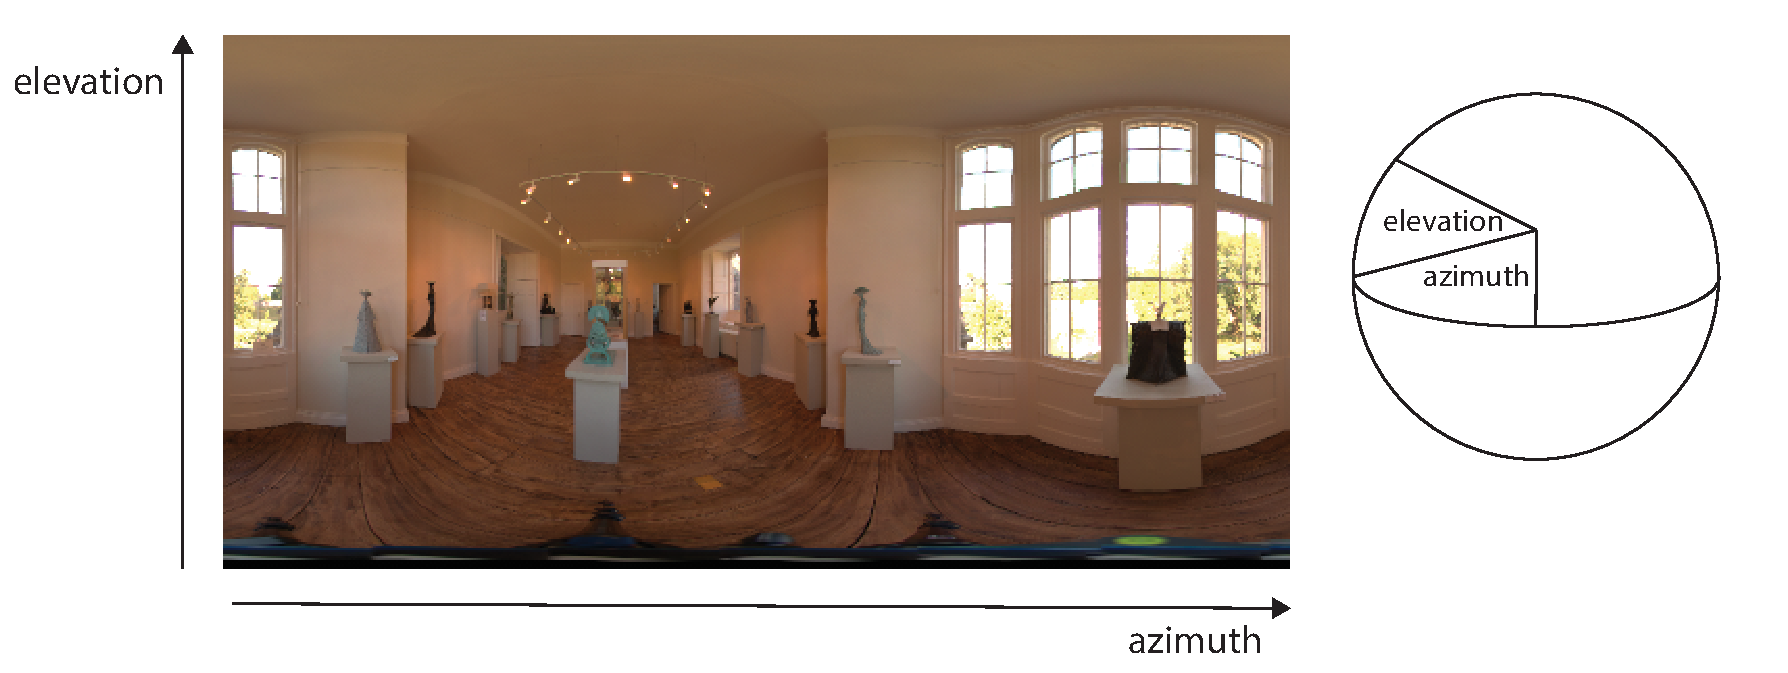
\includegraphics[width=0.6\linewidth]{imgs/envmap.pdf}
    \caption{An environment map is an infinitely far away area light the maps each point on a sphere to a directional light source. (Sorry for the abstract drawing. Hopefully you get the idea.)}
    \label{fig:envmap}
\end{figure}

A diffuse area light should be straightforward: it is attached to some geometry, and emits lights uniformly in all directions. An environment map is usually represented as an image, and emits light on a sphere that is infinitely large (Figure~\ref{fig:envmap}). These two light sources are the most common kind in production. Some renderers implement area lights with spatial-directionally varying properties, but the emission profiles of light sources are more scarce compared to BSDF (which is already scarce) -- more research needed!

All lights in lajolla needs to implement the following functions:
\begin{lstlisting}[language=c++]
/// Computes the total power the light emit to all positions and directions.
/// Useful for sampling.
Real light_power(const Light &light, const Scene &scene);

/// Given some random numbers, sample a point on the light source.
/// If the point is on a surface, returns both the point & normal on it.
/// If the point is infinitely far away (e.g., on an environment map),
/// we store the direction that points towards the origin in PointAndNormal.normal.
/// rnd_param_w is usually used for choosing a discrete element e.g., choosing a triangle in a mesh light.
/// rnd_param_uv is usually used for picking a point on that element.
PointAndNormal sample_point_on_light(const Light &light, 
                                     const PathVertex &vertex,
                                     const Vector2 &rnd_param_uv,
                                     Real rnd_param_w,
                                     const Scene &scene);

/// Given a point on the light source, compute the sampling density for the function above.
Real pdf_point_on_light(const Light &light,
                        const PointAndNormal &point_on_light,
                        const PathVertex &vertex,
                        const Scene &scene);

/// Given a viewing direction pointing outwards from the light, and a point on the light,
/// compute the emission of the light. We also need the "footprint" of the ray
/// for texture filtering. For finite position, view_footprint stores (approximatedly) du/dx
/// and for infinite direction (e.g., envmap), view_footprint stores the approximated ddir/dx.
Spectrum emission(const Light &light,
                  const Vector3 &view_dir,
                  Real view_footprint,
                  const PointAndNormal &point_on_light,
                  const Scene &scene);

/// Some lights require storing sampling data structures inside. This function initialize them.
void init_sampling_dist(Light &light, const Scene &scene);
\end{lstlisting}

Hopefully the comments are self-explanatory (let us know if they are not). I recommend you read the source code of these lights to have a better understanding of what is happening.

\section{Geometry}
A renderer also needs representation of surfaces in the scene. Lajolla supports two kinds of geometry (or \lstinline{Shape}):

\begin{lstlisting}[language=c++]
struct Sphere : public ShapeBase {
    Vector3 position;
    Real radius;
};

struct TriangleMesh : public ShapeBase {
    std::vector<Vector3> positions;
    std::vector<Vector3i> indices;
    std::vector<Vector3> normals;
    std::vector<Vector2> uvs;
    /// Below are used only when the mesh is associated with an area light
    Real total_area;
    /// For sampling a triangle based on its area
    TableDist1D triangle_sampler;
};

using Shape = std::variant<Sphere, TriangleMesh>;
\end{lstlisting}

Lajolla uses \href{https://www.embree.org/}{Embree} as its ray casting engine. So a shape would need to register itself to the Embree API:
\begin{lstlisting}[language=c++]
/// Add the shape to an Embree scene.
uint32_t register_embree(const Shape &shape, const RTCDevice &device, const RTCScene &scene);
\end{lstlisting}

Embree has native support for a triangle mesh, so registering a triangle mesh to Embree is simple:
\begin{lstlisting}[language=c++]
uint32_t register_embree_op::operator()(const TriangleMesh &mesh) const {
    RTCGeometry rtc_geom = rtcNewGeometry(device, RTC_GEOMETRY_TYPE_TRIANGLE);
    // A geomID is the ID associated with the shape inside Embree.
    uint32_t geomID = rtcAttachGeometry(scene, rtc_geom);
    Vector4f *positions = (Vector4f*)rtcSetNewGeometryBuffer(
        rtc_geom, RTC_BUFFER_TYPE_VERTEX, 0, RTC_FORMAT_FLOAT3,
        sizeof(Vector4f), mesh.positions.size());
    Vector3i *triangles = (Vector3i*)rtcSetNewGeometryBuffer(
        rtc_geom, RTC_BUFFER_TYPE_INDEX, 0, RTC_FORMAT_UINT3,
        sizeof(Vector3i), mesh.indices.size());
    for (int i = 0; i < (int)mesh.positions.size(); i++) {
        Vector3 position = mesh.positions[i];
        positions[i] = Vector4f{(float)position[0], (float)position[1], (float)position[2], 0.f};
    }
    for (int i = 0; i < (int)mesh.indices.size(); i++) {
        triangles[i] = mesh.indices[i];
    }
    rtcSetGeometryVertexAttributeCount(rtc_geom, 1);
    rtcCommitGeometry(rtc_geom);
    rtcReleaseGeometry(rtc_geom);
    return geomID;
}
\end{lstlisting}

Registering a sphere is more complicated, since we will need to implement our own ray-sphere intersection routines:
\begin{lstlisting}[language=c++]
void sphere_bounds_func(const struct RTCBoundsFunctionArguments* args);
void sphere_intersect_func(const RTCIntersectFunctionNArguments* args);
void sphere_occluded_func(const RTCOccludedFunctionNArguments* args);

uint32_t register_embree_op::operator()(const Sphere &sphere) const {
    RTCGeometry rtc_geom = rtcNewGeometry(device, RTC_GEOMETRY_TYPE_USER);
    uint32_t geomID = rtcAttachGeometry(scene, rtc_geom);
    rtcSetGeometryUserPrimitiveCount(rtc_geom, 1);
    rtcSetGeometryUserData(rtc_geom, (void *)&sphere);
    rtcSetGeometryBoundsFunction(rtc_geom, sphere_bounds_func, nullptr);
    rtcSetGeometryIntersectFunction(rtc_geom, sphere_intersect_func);
    rtcSetGeometryOccludedFunction(rtc_geom, sphere_occluded_func);
    rtcCommitGeometry(rtc_geom);
    rtcReleaseGeometry(rtc_geom);
    return geomID;
}
\end{lstlisting}

Apart from the Embree registration, we also need to compute relevant information for shading and texture filtering.
\begin{lstlisting}[language=c++]
struct ShadingInfo {
    Vector2 uv; // UV coordinates for texture mapping
    Frame shading_frame; // the coordinate basis for shading
    Real mean_curvature; // 0.5 * (dot(dN/du, shading_frame.x) + dot(dN/dv, shading_frame.y))
    // Stores min(length(dp/du), length(dp/dv)), for ray differentials.
    Real inv_uv_size;
};

ShadingInfo compute_shading_info(const Shape &shape, const PathVertex &vertex);
\end{lstlisting}
All of these quantities can be computed using elementary differential geometry. You should read the source code if you are interested.

Finally, a shape also needs to implement some other sampling routines for area light sampling:
\begin{lstlisting}[language=c++]
/// Sample a point on the surface
PointAndNormal sample_point_on_shape(const Shape &shape,
                                     const PathVertex &vertex,
                                     const Vector2 &uv,
                                     Real w);

/// Probability density of the operation above
Real pdf_point_on_shape(const Shape &shape,
                        const PointAndNormal &point_on_shape,
                        const PathVertex &vertex);

/// Useful for sampling.
Real surface_area(const Shape &shape);

/// Some shapes require storing sampling data structures inside. This function initialize them.
void init_sampling_dist(Shape &shape);
\end{lstlisting}

\section{Utilities and miscellaneous topics}

\subsection{Vectors}
Lajolla uses its own N-d vector implementations:
\begin{lstlisting}[language=c++]
template <typename T>
struct TVector2 {
    // ...
    T& operator[](int i) {
        return *(&x + i);
    }
    T operator[](int i) const {
        return *(&x + i);
    }
    T x, y;
};

template <typename T>
struct TVector3 {
    // ...
    T& operator[](int i) {
        return *(&x + i);
    }
    T operator[](int i) const {
        return *(&x + i);
    }
    T x, y, z;
};

template <typename T>
struct TVector4 {
    // ...
    T& operator[](int i) {
        return *(&x + i);
    }
    T operator[](int i) const {
        return *(&x + i);
    }
    T x, y, z, w;
};
using Vector2 = TVector2<Real>;
using Vector3 = TVector3<Real>;
using Vector4 = TVector4<Real>;
\end{lstlisting}

We use operator overloading to support common vector operations
(\lstinline{+}, \lstinline{-}, \lstinline{*}, \lstinline{/}, \lstinline{dot}, \lstinline{cross}, \lstinline{length},
\lstinline{distance}, \lstinline{normalize}, etc). Not all operations are implemented for everything, so
you might need to implement some for your own convienence.

\subsection{Matrices}
Lajolla implements a 4x4 row-major matrix with hard-coded inversion and matrix-matrix multiplication. 
\begin{lstlisting}[language=c++]
template <typename T>
struct TMatrix4x4 {
    const T& operator()(int i, int j) const {
        return data[i][j];
    }

    T& operator()(int i, int j) {
        return data[i][j];
    }

    static TMatrix4x4<T> identity() {
        TMatrix4x4<T> m(1, 0, 0, 0,
                        0, 1, 0, 0,
                        0, 0, 1, 0,
                        0, 0, 0, 1);
        return m;
    }

    T data[4][4];
}
\end{lstlisting}

To use these matrices to transform points, vectors, and normals, use the following functions:
\begin{lstlisting}[language=c++]
Vector3 xform_point(const Matrix4x4 &xform, const Vector3 &pt);
Vector3 xform_vector(const Matrix4x4 &xform, const Vector3 &vec);
Vector3 xform_normal(const Matrix4x4 &inv_xform, const Vector3 &n);
\end{lstlisting}

To build a matrix from a common 3D transformation, use the following functions:
\begin{lstlisting}[language=c++]
Matrix4x4 translate(const Vector3 &delta);
Matrix4x4 scale(const Vector3 &scale);
Matrix4x4 rotate(Real angle, const Vector3 &axis);
Matrix4x4 look_at(const Vector3 &pos, const Vector3 &look, const Vector3 &up);
Matrix4x4 perspective(Real fov);
\end{lstlisting}

\subsection{Color and Spectrum}
Spectral rendering is a complicated topic and requires its own document (see \href{https://www.csie.ntu.edu.tw/~cyy/courses/rendering/16fall/lectures/handouts/chap05_color_radiometry.pdf}{these slides} from my undergraduate institution for a really nice introduction to color and radiometry). In principle, while
it is sufficient to use RGB representing color on an image, it is insufficient to just use RGB
to represent reflectance and emission, since the interaction between photons and reflectance at different
wavelengths will affect the final RGB values non-linearly. Unfortunately, spectral measurement of materials is scarce (more research!) and most textures we have are on RGB format. For this reason, we still opt for an RGB representation
of the spectrum. There are production renderers that support full spectral rendering. Manuka is a notable example~\cite{Fascione:2018:MBA}.

\begin{lstlisting}[language=c++]
/// For now, lajolla assumes we are operating in the linear and trimulus RGB color space.
/// In the future we might implement a proper spectral renderer.
using Spectrum = Vector3;

inline Spectrum make_zero_spectrum() {
    return Vector3{0, 0, 0};
}

inline Spectrum make_const_spectrum(Real v) {
    return Vector3{v, v, v};
}

inline Spectrum fromRGB(const Vector3 &rgb) {
    return rgb;
}

inline Spectrum sqrt(const Spectrum &s) {
    return Vector3{sqrt(max(s[0], Real(0))),
                   sqrt(max(s[1], Real(0))),
                   sqrt(max(s[2], Real(0)))};
}

inline Real luminance(const Spectrum &s) {
    return s.x * Real(0.212671) + s.y * Real(0.715160) + s.z * Real(0.072169);
}
\end{lstlisting}

To render some Mitsuba scenes, we need to convert spectral data to RGB. We use a curve-fitting solution from Wyman et al. for doing so~\cite{Wyman:2013:SAP}.
\begin{lstlisting}[language=c++]
inline Real xFit_1931(Real wavelength) {
    Real t1 = (wavelength - Real(442.0)) * ((wavelength < Real(442.0)) ? Real(0.0624) : Real(0.0374));
    Real t2 = (wavelength - Real(599.8)) * ((wavelength < Real(599.8)) ? Real(0.0264) : Real(0.0323));
    Real t3 = (wavelength - Real(501.1)) * ((wavelength < Real(501.1)) ? Real(0.0490) : Real(0.0382));
    return Real(0.362) * exp(-Real(0.5) * t1 * t1) + 
           Real(1.056) * exp(-Real(0.5) * t2 * t2) -
           Real(0.065) * exp(-Real(0.5) * t3 * t3);
}
inline Real yFit_1931(Real wavelength) {
    Real t1 = (wavelength - Real(568.8)) * ((wavelength < Real(568.8)) ? Real(0.0213) : Real(0.0247));
    Real t2 = (wavelength - Real(530.9)) * ((wavelength < Real(530.9)) ? Real(0.0613) : Real(0.0322));
    return Real(0.821) * exp(-Real(0.5) * t1 * t1) +
           Real(0.286) * exp(-Real(0.5) * t2 * t2);
}
inline Real zFit_1931(Real wavelength) {
    Real t1 = (wavelength - Real(437.0)) * ((wavelength < Real(437.0)) ? Real(0.0845) : Real(0.0278));
    Real t2 = (wavelength - Real(459.0)) * ((wavelength < Real(459.0)) ? Real(0.0385) : Real(0.0725));
    return Real(1.217) * exp(-Real(0.5) * t1 * t1) +
           Real(0.681) * exp(-Real(0.5) * t2 * t2);
}
inline Vector3 XYZintegral_coeff(Real wavelength) {
    return Vector3{xFit_1931(wavelength), yFit_1931(wavelength), zFit_1931(wavelength)};
}

inline Vector3 integrate_XYZ(const std::vector<std::pair<Real, Real>> &data) {
    static const Real CIE_Y_integral = 106.856895;
    static const Real wavelength_beg = 400;
    static const Real wavelength_end = 700;
    if (data.size() == 0) {
        return Vector3{0, 0, 0};
    }
    Vector3 ret = Vector3{0, 0, 0};
    int data_pos = 0;
    // integrate from wavelength 400 nm to 700 nm, increment by 1nm at a time
    // linearly interpolate from the data
    for (Real wavelength = wavelength_beg; wavelength <= wavelength_end; wavelength += Real(1)) {
        // assume the spectrum data is sorted by wavelength
        // move data_pos such that wavelength is between two data or at one end
        while(data_pos < data.size() - 1 &&
               !((data[data_pos].first <= wavelength &&
                  data[data_pos + 1].first > wavelength) ||
                 data[0].first > wavelength)) {
            data_pos += 1;
        }
        Real measurement = 0;
        if (data_pos < data.size() - 1 && data[0].first <= wavelength) {
            Real curr_data = data[data_pos].second;
            Real next_data = data[std::min(data_pos + 1, (int)data.size() - 1)].second;
            Real curr_wave = data[data_pos].first;
            Real next_wave = data[std::min(data_pos + 1, (int)data.size() - 1)].first;
            // linearly interpolate
            measurement = curr_data * (next_wave - wavelength) / (next_wave - curr_wave) +
                          next_data * (wavelength - curr_wave) / (next_wave - curr_wave);
        } else {
            // assign the endpoint
            measurement = data[data_pos].second;
        }
        Vector3 coeff = XYZintegral_coeff(wavelength);
        ret += coeff * measurement;
    }
    Real wavelength_span = wavelength_end - wavelength_beg;
    ret *= (wavelength_span / (CIE_Y_integral * (wavelength_end - wavelength_beg)));
    return ret;
}
inline Vector3 XYZ_to_RGB(const Vector3 &xyz) {
    return Vector3{
        Real( 3.240479) * xyz[0] - Real(1.537150) * xyz[1] - Real(0.498535) * xyz[2],
        Real(-0.969256) * xyz[0] + Real(1.875991) * xyz[1] + Real(0.041556) * xyz[2],
        Real( 0.055648) * xyz[0] - Real(0.204043) * xyz[1] + Real(1.057311) * xyz[2]};
}
\end{lstlisting}

\subsection{Frame}

A Frame is a 3D coordinate system with an orthonormal basis $(x, y, n)$.
\begin{lstlisting}[language=c++]
/// A "Frame" is a coordinate basis that consists of three orthogonal unit vectors.
/// This is useful for sampling points on a hemisphere or defining anisotropic BSDFs.
struct Frame {
    Frame() {}

    Frame(const Vector3 &x, const Vector3 &y, const Vector3 &n)
        : x(x), y(y), n(n) {}

    Frame(const Vector3 &n) : n(n) {
        std::tie(x, y) = coordinate_system(n);
    }

    inline Vector3& operator[](int i) {
        return *(&x + i);
    }
    inline const Vector3& operator[](int i) const {
        return *(&x + i);
    }
    Vector3 x, y, n;
};
\end{lstlisting}

It is useful to have a way to construct a frame from only the normal (z) vector. We use the method
from Frisvad that is numerically stable~\cite{Frisvad:2012:BOB}:
\begin{lstlisting}[language=c++]
/// Given a vector n, outputs two vectors such that all three vectors are
/// orthogonal to each other.
/// The approach here is based on Frisvad's paper
/// "Building an Orthonormal Basis from a 3D Unit Vector Without Normalization"
/// https://backend.orbit.dtu.dk/ws/portalfiles/portal/126824972/onb_frisvad_jgt2012_v2.pdf
inline std::pair<Vector3, Vector3> coordinate_system(const Vector3 &n) {
    if (n[2] < Real(-1 + 1e-6)) {
        return std::make_pair(Vector3{0, -1, 0},
                              Vector3{-1, 0, 0});
    } else {
        Real a = 1 / (1 + n[2]);
        Real b = -n[0] * n[1] * a;
        return std::make_pair(Vector3{1 - n[0] * n[0] * a, b, -n[0]},
                              Vector3{b, 1 - n[1] * n[1] * a, -n[1]});
    }
}
\end{lstlisting}

\subsection{Parallelization}
We take the parallelization code from \href{https://github.com/mmp/pbrt-v3/blob/master/src/core/parallel.h}{pbrt}. The following functions can be used for parallelizing loops:
\begin{lstlisting}[language=c++]
void parallel_for(const std::function<void(int64_t)> &func, int64_t count, int64_t chunkSize = 1);
void parallel_for(std::function<void(Vector2i)> func, const Vector2i count);
\end{lstlisting}

For example, the main rendering loop looks like this
\begin{lstlisting}[language=c++]
constexpr int tile_size = 16;
int num_tiles_x = (w + tile_size - 1) / tile_size;
int num_tiles_y = (h + tile_size - 1) / tile_size;

ProgressReporter reporter(num_tiles_x * num_tiles_y);
parallel_for([&](const Vector2i &tile) {
    // Use a different rng stream for each thread.
    pcg32_state rng = init_pcg32(tile[1] * num_tiles_x + tile[0]);
    int x0 = tile[0] * tile_size;
    int x1 = min(x0 + tile_size, w);
    int y0 = tile[1] * tile_size;
    int y1 = min(y0 + tile_size, h);
    for (int y = y0; y < y1; y++) {
        for (int x = x0; x < x1; x++) {
            Spectrum radiance = make_zero_spectrum();
            int spp = scene.options.samples_per_pixel;
            for (int s = 0; s < spp; s++) {
                radiance += path_tracing(scene, x, y, rng);
            }
            img(x, y) = radiance / Real(spp);
        }
    }
    reporter.update(1);
}, Vector2i(num_tiles_x, num_tiles_y));
\end{lstlisting}

\subsection{Random number generation}
Lajolla uses a random number generator called \href{https://www.pcg-random.org/}{PCG} which is a very lightweight random number generator based on simple postprocessing of a standard linear congruent generator. PCG generally has good statistical properties and is much cheaper to compute compared to more advanced RNG, e.g., Merserner Twister. Highly recommend Melissa O'Neill's \href{https://www.youtube.com/watch?v=45Oet5qjlms}{talk} about PCG.

A crucial feature of PCG is that it allows multiple "streams": given a seed, we can initialize many different streams of RNGs that have different independent random numbers.

\begin{lstlisting}[language=c++]
inline pcg32_state init_pcg32(uint64_t stream_id = 1, uint64_t seed = 0x853c49e6748fea9bULL);
T next_pcg32_real(pcg32_state &rng);
\end{lstlisting}

\paragraph{Stratification.} Independent random numbers are in fact not a really good choice for Monte Carlo rendering. Samples can be clumped together and not provide good coverage of the sampling space. Stratified random sampling or low-discrepancy sequences are much better choices. We do not implement these in lajolla (final project idea!), but we will cover them in the class.

\subsection{Reusing random numbers}
A commonly encountered scenario is when we only have one random number, but we want to use it for two random choices (we don't want to generate a new random number because it breaks the stratification property). If the first random choice we made is a discrete choice, this is possible. Consider the case where we want to sample one between two components of a BSDF, then sample an outgoing direction. Choosing between the two components only consumes 1-bit of the random numbers, and we still have 31/63 bits left depending on the floating-point representation we use. Thus, we can remap the random number to reuse it. 
\begin{lstlisting}[language=c++]
Real u = ...; // uniform random number
Real prob = ...;
if (u < prob) {
    // remap u from [0, prob) to [0, 1]
    u = u / prob;
    return f(u);
} else {
    // remap u from [prob, 1] to [0, 1]
    u = (u - prob) / (1 - prob);
    return g(u);
}
\end{lstlisting}

You might need to do this in homework 1!

\subsection{Table distributions}
We often need to sample from a discrete distribution (e.g., picking a light source), or a piecewise-constant continuous distribution (e.g., an environment map).
\lstinline{TableDist1D} implements a 1D discrete distribution, and \lstinline{TableDist2D} implements a 2D piecewise constant distribution.
\begin{lstlisting}[language=c++]
/// TableDist1D stores a tabular discrete distribution
/// that we can sample from using the functions below.
/// Useful for light source sampling.
struct TableDist1D {
    std::vector<Real> pmf;
    std::vector<Real> cdf;
};

/// Construct the tabular discrete distribution given a vector of positive numbers.
TableDist1D make_table_dist_1d(const std::vector<Real> &f);
/// Sample an entry from the discrete table given a random number in [0, 1]
int sample(const TableDist1D &table, Real rnd_param);
/// The probability mass function of the sampling procedure above.
Real pmf(const TableDist1D &table, int id);

/// TableDist2D stores a 2D piecewise constant distribution
/// that we can sample from using the functions below.
/// Useful for envmap sampling.
struct TableDist2D {
    // cdf_rows & pdf_rows store a 1D piecewise constant distribution
    // for each row.
    std::vector<Real> cdf_rows, pdf_rows;
    // cdf_maringlas & pdf_marginals store a single 1D piecewise
    // constant distribution for sampling a row
    std::vector<Real> cdf_marginals, pdf_marginals;
    Real total_values;
    int width, height;
};

/// Construct the 2D piecewise constant distribution given a vector of positive numbers
/// and width & height.
TableDist2D make_table_dist_2d(const std::vector<Real> &f, int width, int height);
/// Given two random number in [0, 1]^2, sample a point in the 2D domain [0, 1]^2
/// with distribution proportional to f above.
Vector2 sample(const TableDist2D &table, const Vector2 &rnd_param);
/// Probability density of the sampling procedure above.
Real pdf(const TableDist2D &table, const Vector2 &xy);
\end{lstlisting}

Sampling from a 1D distribution can be done using a binary search to invert the CDF. Sampling
from a 2D distribution with size $(w, h)$ can be done using $h$ 1D distribution to sample each row,
and use one more 1D distribution to sample a column based on their marginal distribution.

See the pbrt book for more explaination: \href{https://pbr-book.org/3ed-2018/Monte_Carlo_Integration/Sampling_Random_Variables#x1-Example:Piecewise-Constant1DFunctions}{for 1D distributions}, and \href{https://www.pbr-book.org/3ed-2018/Monte_Carlo_Integration/2D_Sampling_with_Multidimensional_Transformations#Piecewise-Constant2DDistributions}{for 2D distributions}.

\subsection{Russian roulette}

The rendering equation recurses indefintely and can lead to infinite loops. We need to truncate the loop at some point, but an arbitrary truncate can lead to energy loss. The trick is to truncate the path \emph{probabilistically}, then scale the contribution by the inverse probability if the path does not terminate. This ``Russian roulette'' trick was originated for nuclear engineering simulation. Arvo and Kirk brought this idea to graphics in 1990~\cite{Arvo:1990:PTI}. Determining a good path truncation probability is hard~\cite{Vorba:2016:ARR}. We just use a very basic heuristics based on the path throughput and the index of refraction.

\begin{lstlisting}
Real rr_prob = 1;
if (num_vertices + 1 >= scene.options.rr_depth) {
    rr_prob = min(max((1 / eta_scale) * current_path_throughput), Real(0.95));
    if (next_pcg32_real<Real>(rng) > rr_prob) {
        // Terminate the path
        break;
    }
}
current_path_throughput = current_path_throughput * (G * f) / (p2 * rr_prob);
\end{lstlisting}

\bibliographystyle{plain}
\bibliography{refs}

\end{document}
